
\documentclass[11pt]{article}

\usepackage{listings}
\usepackage{graphicx}
\usepackage{amsmath}
\usepackage{amsfonts}
\usepackage{amssymb}
\usepackage{pgfgantt}
\usepackage{amsthm}
\usepackage{fancyhdr}
\usepackage{rotating}
\usepackage[graphicx]{realboxes}
\renewcommand{\vec}{\bm}
\usepackage{dsfont}
\usepackage{xcolor}
\usepackage{sectsty}
\usepackage{pdflscape}

\usepackage[paper=a4paper,top=0.4in,left=0.5in, right=0.5in, bottom=0.4in]{geometry}
\definecolor{lightorange}{RGB}{251,211,168}
\definecolor{darkred}{RGB}{153,0,0}
\definecolor{darkgreen}{RGB}{0,51,25}
\definecolor{gray}{RGB}{32,32,32}

\sectionfont{\fontsize{12}{15}\selectfont}
\newcounter{myWeekNum}
\stepcounter{myWeekNum}
%
\newcommand{\myWeek}{\themyWeekNum
    \stepcounter{myWeekNum}
    \ifnum\themyWeekNum=16
    \setcounter{myWeekNum}{1}
    \else\fi
}
%

\begin{document}
\begin{landscape}
  \thispagestyle{empty}
  \setcounter{myWeekNum}{1}
    \ganttset{%
        calendar week text={\myWeek{}}%
    }
  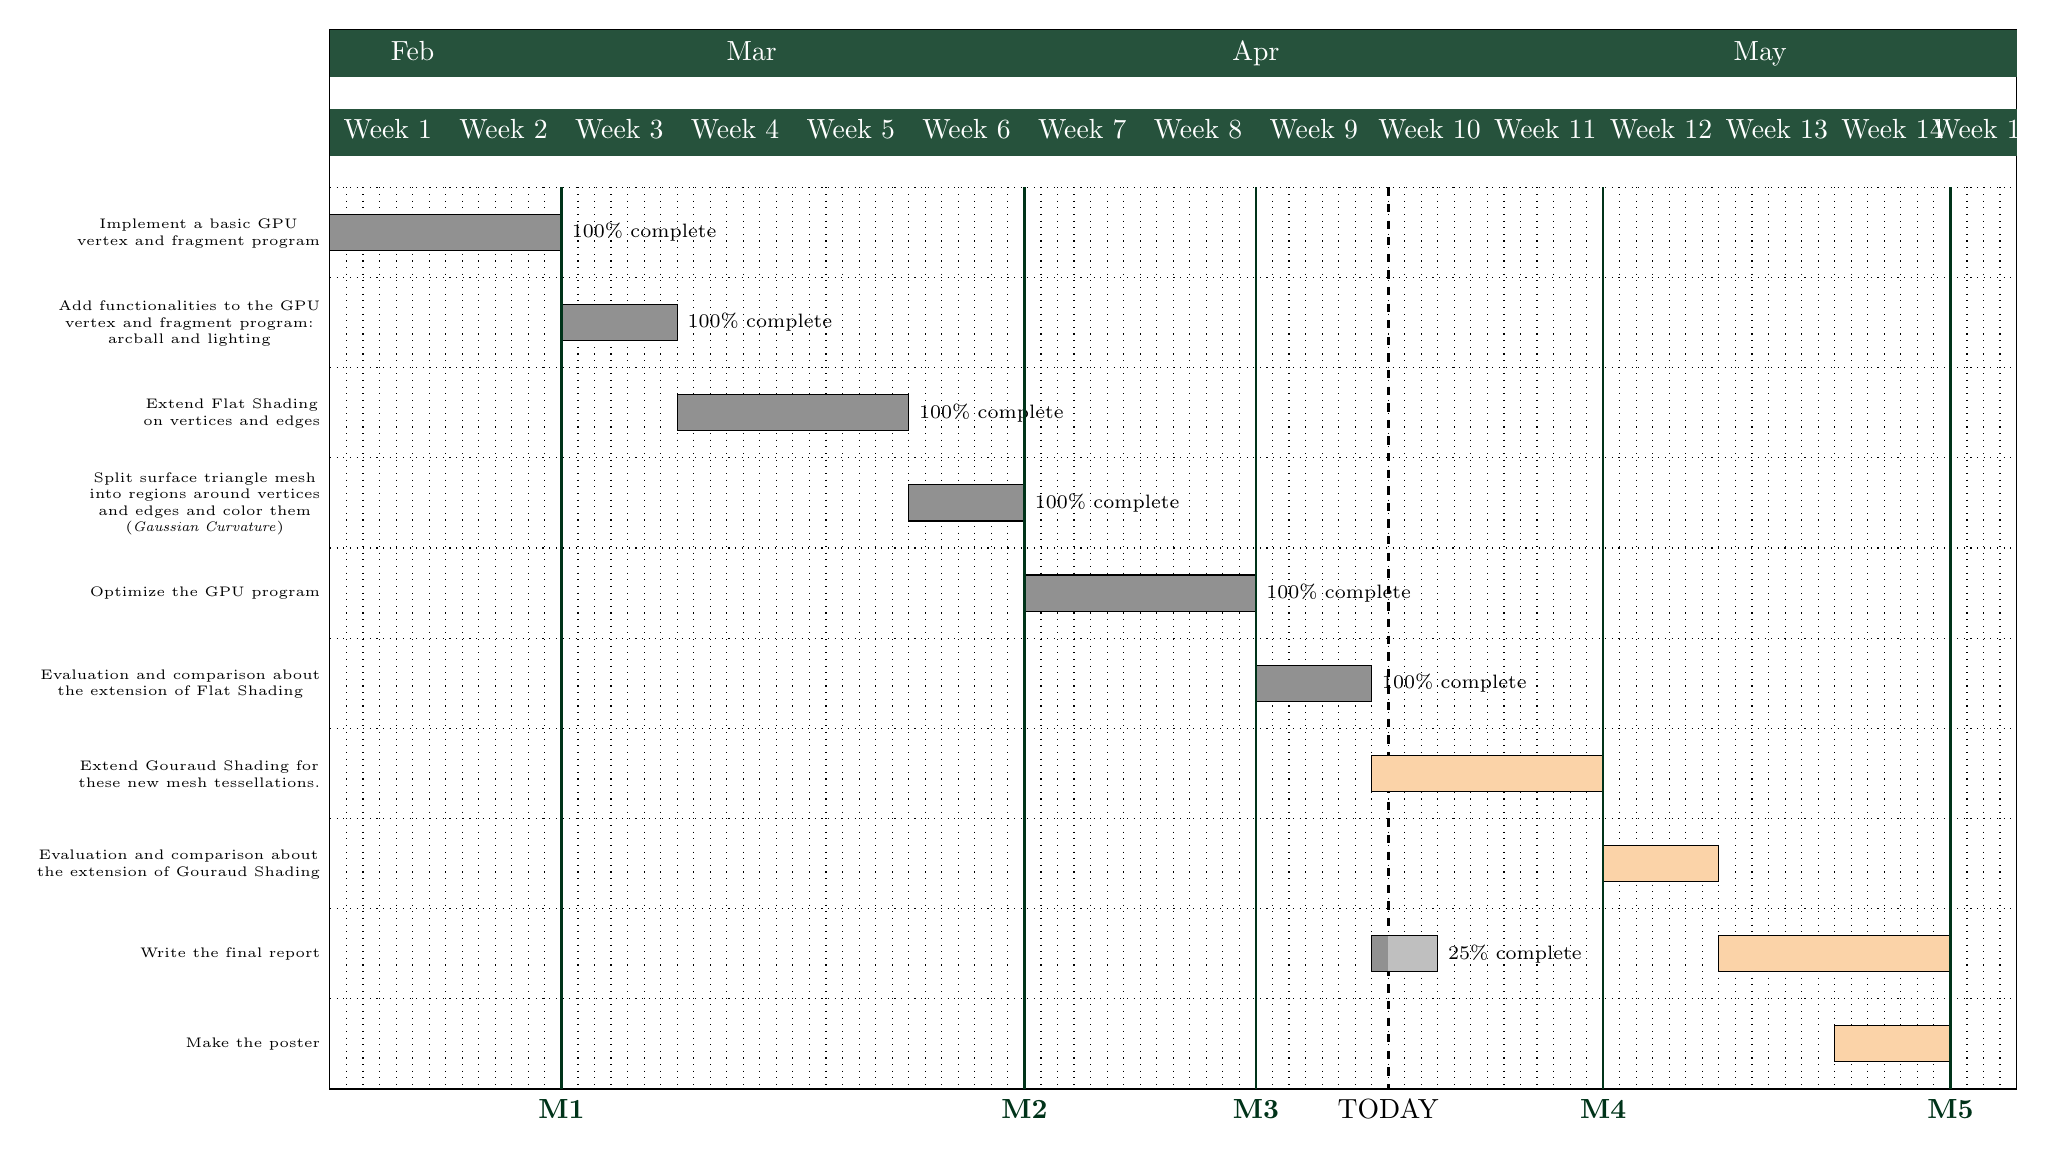
\begin{tikzpicture}
  % \begin{rotate}{270}
  % \noindent\resizebox{\textwidth}{!}{
      % \begin{ganttchart}[vgrid, hgrid, bar/.append style={fill=lightorange}, link/.style={-latex, draw=darkred, fill=darkred},vrule/.style={thick, darkgreen},
      %   vrule label font=\bfseries]{1}{28}
      \begin{ganttchart}[
        hgrid,
        vgrid,
        title/.style={fill=darkgreen!85, draw=none},
        title label font=\color{white},
        bar height=.4,
        bar/.append style={fill=lightorange},
        bar label node/.append style={align=center, font=\tiny},
        bar label font=\normalsize\color{black!100},
        % bar incomplete/.append style={fill=lightorange},
        vrule/.style={thick, darkgreen},
        vrule label font=\bfseries,
        x unit=2.1mm,
        y unit chart=1.145cm,
        time slot format=little-endian,
        % progress=today,
        today=23.4.18
        ]{19.2.2018}{31.5.2018}
  \gantttitlecalendar*{19.2.2018}{31.5.2018}{month=shortname, week} \\
  \ganttbar[
    progress=100,
    bar/.append style={fill=black!43}
    ]{Implement a basic GPU\ganttalignnewline vertex and fragment program}{19.2.2018}{4.3.2018} \\
  \ganttbar[
    progress=100,
    bar/.append style={fill=black!43}
    ]{Add functionalities to the GPU\ganttalignnewline vertex and fragment program:\ganttalignnewline arcball and lighting}{5.3.2018}{11.3.2018} \\
  \ganttbar[
    progress=100,
    bar/.append style={fill=black!43}
    ]{Extend Flat Shading\ganttalignnewline on vertices and edges}{12.3.2018}{25.3.2018} \ganttnewline
  \ganttbar[
    progress=100,
    bar/.append style={fill=black!43}
    ]{Split surface triangle mesh\ganttalignnewline into regions around vertices\ganttalignnewline and edges and color them \ganttalignnewline (\textit{Gaussian Curvature})}{26.3.2018}{01.4.2018} \ganttnewline
  \ganttbar[
    progress=100,
    bar/.append style={fill=black!43}
  ]{Optimize the GPU program}{02.4.2018}{15.4.2018} \ganttnewline
  \ganttbar[
    progress=100,
    bar/.append style={fill=black!43}
  ]{Evaluation and comparison about\ganttalignnewline the extension of Flat Shading}{16.4.2018}{22.4.2018} \ganttnewline
  \ganttbar{Extend Gouraud Shading for\ganttalignnewline these new mesh tessellations.}{23.4.2018}{6.5.2018} \ganttnewline
  \ganttbar{Evaluation and comparison about\ganttalignnewline the extension of Gouraud Shading }{7.5.2018}{13.5.2018} \ganttnewline
  \ganttbar{Write the final report}{14.5.2018}{27.5.2018}
  \ganttbar[
    progress=25,
    bar/.append style={fill=black!43}
  ]{}{23.4.2018}{26.4.2018}
  \ganttnewline
  \ganttbar{Make the poster}{21.5.2018}{27.5.2018}
  \ganttvrule{M1}{04.03.2018}
  \ganttvrule{M2}{01.4.2018}
  \ganttvrule{M3}{15.4.2018}
  \ganttvrule{M4}{6.5.2018}
  \ganttvrule{M5}{27.5.2018}
\end{ganttchart}
\end{tikzpicture}
\begin{itemize}
  \item [] \textbf{Milestone 1:} A first version of the GPU vertex program that loads a mesh and colors it using a vertex based area.
  \item [] \textbf{Milestone 2:} Implementation of Flat shading on vertices and edges.
  \item [] \textbf{Milestone 3:} GPU fragment program.
  \item [] \textbf{Milestone 4:} Implementation of an extension of Gouraud shading.
  \item [] \textbf{Milestone 5:} A first version of the report and poster.
\end{itemize}
\begin{flushright}\small{\color{gray!50}{The 15th week will be used only for possible delays or reviews.} \color{darkred}{Red bars mean \textit{Late}.} \color{darkgreen}{Green bars mean \textit{Early}.}}\end{flushright}
\end{landscape}
\end{document}

